%!TEX root = /home/renaud/Documents/EPL/tfe/latex/tfe.tex
\addcontentsline{toc}{chapter}{Introduction}
\chapter*{Introduction}
The understanding of geophysical and environmental fluid flows has shown an increasing interest over the past decades. Climate change, and the related increasing issue of pollution have raised the need for accurate simulations allowing to understand and predict the time-space evolution of the concentration of pollutants in the environment. In this regard, the fate of constituents dissolved in a fluid mixture is commonly modelled by means of reactive-transport equations. Those are coupled partial differential equations taking into account the influence of \textit{reactions} as well as of the advective and diffusive \textit{transport phenomena} on the concentration of the constituent in the mixture. Accurate algorithms have been developed by engineers to numerically solve such equations. Finite differences, finite volume and finite elements methods are amongst the most commonly used discretization methods. However, they rely on grids containing thousands and in some instances millions of grid points so that CPU time can become prohibitive in cases where long time simulations are needed. Furthermore, although those methods provide pretty accurate results, these often suffer from a lack of \textit{interpretation}. This raises the need for simpler models with a few number of variables that would allow for an easier interpretation of the results as well as for fast long time simulations. Obviously, one cannot expect such models to provide results that would be as accurate as the ones furnished by the previously mentioned methods. Hence, both approaches are complementary. 

One way to build such coarser models is to partition the domain of interest into a relatively small number of subdomains, called \textit{compartments} or \textit{boxes} over which the state variables are assumed \textit{homogeneous}. The fluxes between the compartments are then expressed by simple laws, leading to models that are relatively easy to interpret. This procedure leads to models called \textit{compartment models} or equivalently \textit{box models}. The number of subdomains and their shapes vary widely from one problem to another. Some schematic representations of compartment models found in the literature are shown in figure~\ref{fig:intro:boxmodels}.

Box models have been widely used in studies involving marine systems as well at local scale \cite{deleersnijder1998two,maderich2014regional,soetaert1995estimating} as at global scale \cite{kohler2005quantitative,munhoven1996glacial}. The choice of the subdomains and the specification of the fluxes exchanged between them rely on ad-hoc or empirical methods, based on the known hydrodynamics over the domain considered. It seems that no automatic procedure exists to define a relevant partitioning of the domain. The goal of this work is thus to fill that gap by proposing a method based on the tools of \textit{network science} to automatically delineate relevant compartments.

Network science may be defined as the study of graphs (or networks) and their use to model various (real-life or not) problems. Informally, a graph is a mathematical representation of a set of objects (the \textit{nodes} or \textit{vertices} of the graph), and the links between pairs of them (the \textit{edges} of the graph). The field of application of network science is extremely large, as illustrated by this quote from Newman \cite{newman2010networks}: "\textit{Many objects of interest in the physical, biological, and social sciences can be thought of as networks and [...] thinking of them in this way can often lead to new and useful insights}."

Often, graphs exhibit a \textit{community structure}: it is the case if the vertices can be organized into groups such that there are many interactions between the nodes within a group, and few interaction between the nodes of different groups. Such groups of vertices are called \textit{communities} or \textit{clusters}. An example of a three communities partitioning of a simple graph is shown in figure~\ref{fiug:intro:communities}. The art of revealing the community structure of a graph has a long history in network science, and a variety of \textit{community detection algorithms} and \textit{heuristics} has been developed, see \cite{fortunato2010community} for a 2010 survey. Clustering methods have shown to be useful for a wide applications such as social and biological networks \cite{girvan2002community}, biochemical networks \cite{holme2003subnetwork,guimera2005functional,palla2005uncovering}, or informations networks such as the world wide web \cite{flake2002self}. What makes communities particularly appealing is that they often correspond to \textit{functional units} such as cycles or pathways in metabolic networks \cite{guimera2005functional,palla2005uncovering,huss2007currency} or collections of pages on a single topic on the web \cite{flake2002self}. In this work, we aim to show that they also correspond to relevant compartments in the case of advection-diffusion flow networks. We focus on one relatively recent method for community detection based on the \textit{stability} measure \cite{delvenne2010stability,delvenne2013stability,lambiotte2009laplacian}.

A complete procedure is proposed to build a compartment model from any problem whose velocity field and diffusivity tensor are known. First, the Lagrangian equations describing individual particles trajectories are derived from the transport model, and adapted numerical methods are developed. This allows to compute the transition probability matrix at the desired times, which is the information needed to apply the stability clustering method. Finally subdomains are delineated from the communities found by the clustering algorithm, and the exchange coefficients between the compartments are estimated numerically, completing the construction of the box model. This whole procedure is applied on a simple, two dimensional test problem, and the resulting box model is assessed.  

The first part of the work gather all the theoretical tools needed for that procedure. Chapter~\ref{chap:clustering} is devoted to community detection and in particular to the \textit{stability} measure and the related community detection algorithm. The reactive transport equation and the study of its properties is the topic of chapter~\ref{chap:transportmodel}, whereas compartment models and their properties are studied in chapter~\ref{chap:compartment}. Then, the link between the transport model and the Lagrangian equations described the position of an individual particle is shown in chapter~\ref{chap:numerical}, leading to the theory of stochastic differential equations and the consistent numerical methods to solve them. The second part of this work consists in applying the procedure on a simple problem. An idealized, two-dimensional overturning circulation model is presented in~\ref{chap:overturnercirculation} and is then used the build the test problem in chapter~\ref{chap:bioverturner}. The complete procedure is applied on that test problem and assessed in the same chapter. 


\begin{figure}[!htp]
	\begin{subfigure}[t]{.47\linewidth}
		\centering
		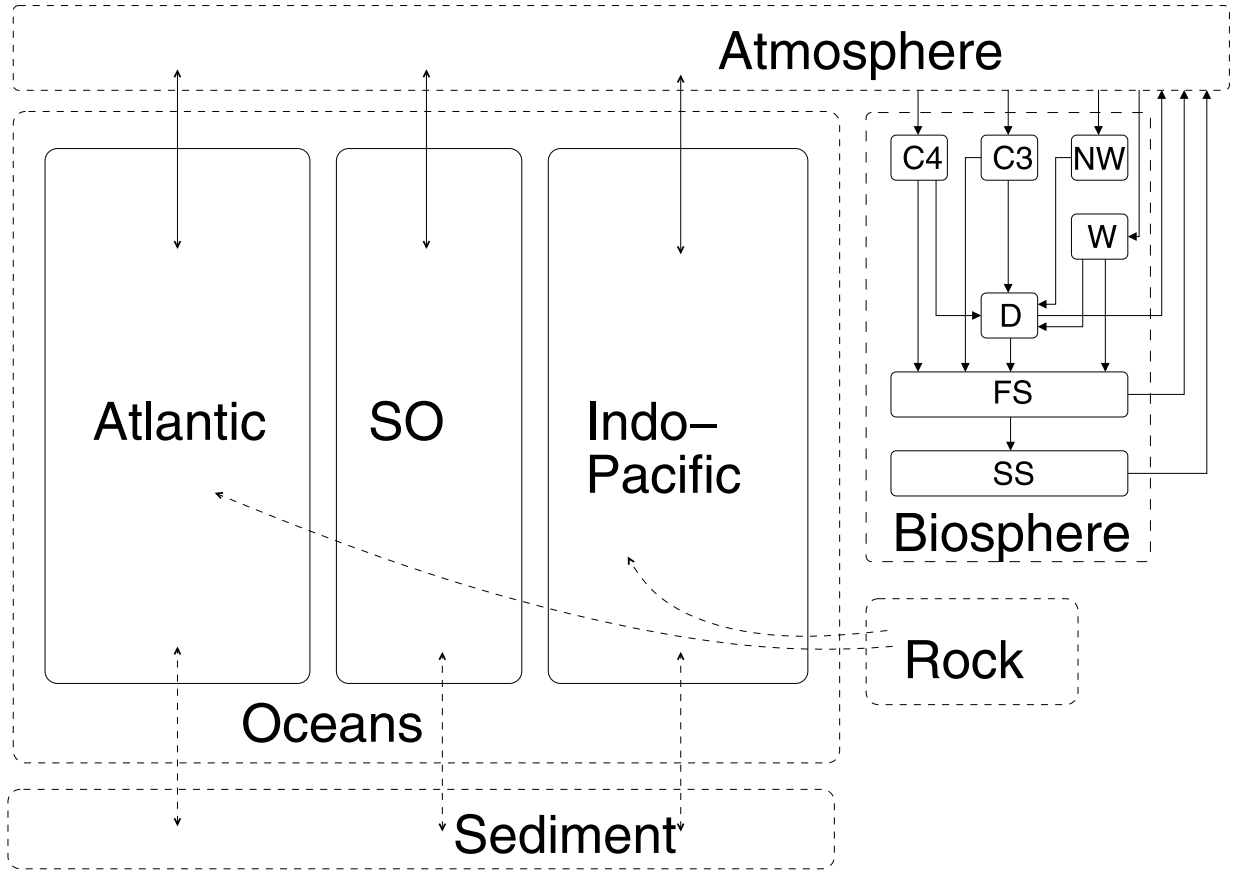
\includegraphics[width=\textwidth]{fig/intro/boxmodel_KohlerEtAl.png}
		\caption{Geometry of the box model of the isotopic carbon cycle (BICYCLE), where the arrows represent carbon fluxes between the compartments. This is figure 1 of \cite{kohler2005quantitative}.}
	\end{subfigure}
		\begin{subfigure}[t]{.51\linewidth}
		\centering
		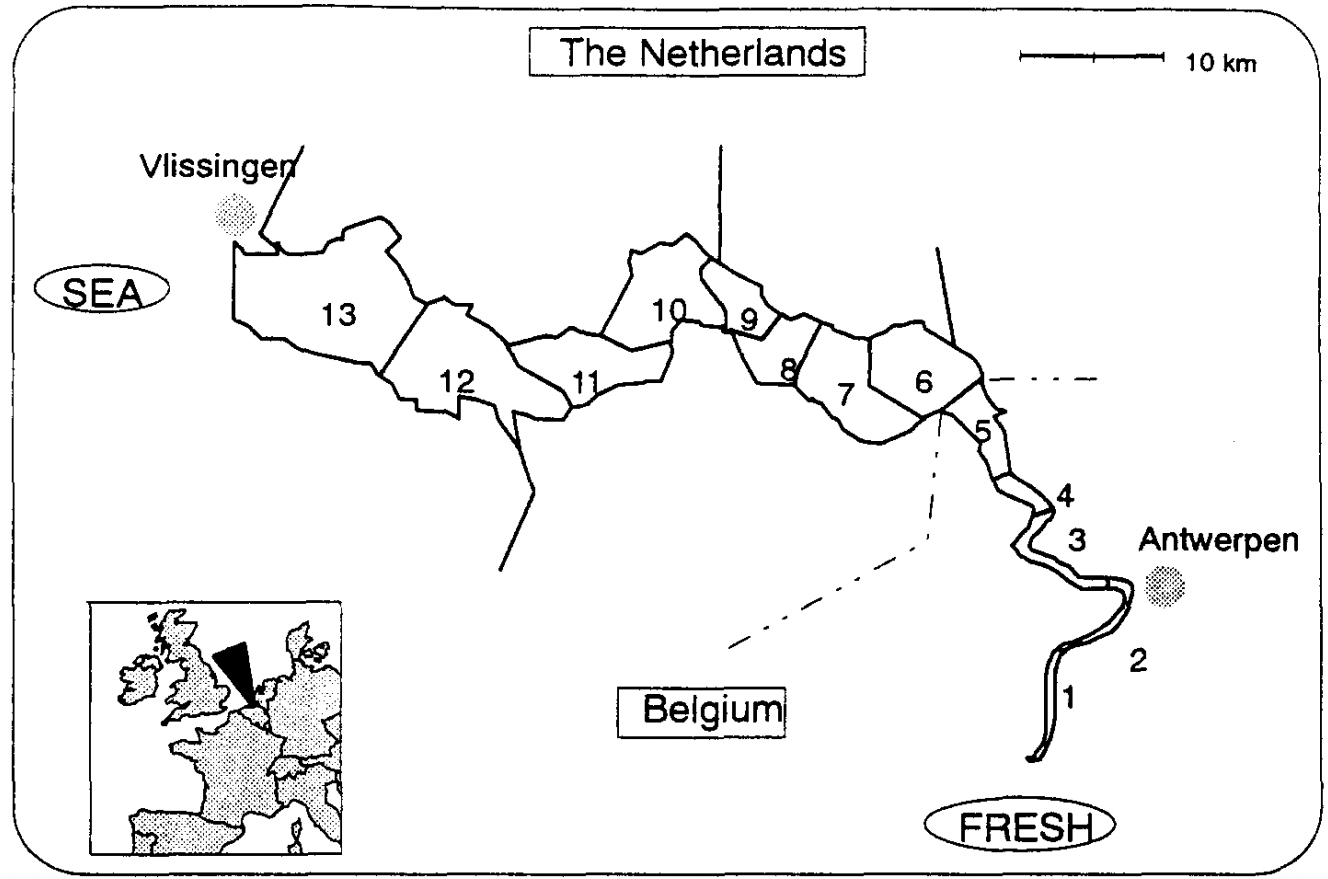
\includegraphics[width=\textwidth]{fig/intro/boxmodel_SoetaertHerman.png}
		\caption{Representation of a subdomain decomposition of the Westerschelde. This is figure 1 of \cite{soetaert1995estimating}.}
	\end{subfigure}
	\begin{subfigure}[b]{\linewidth}
		\centering
		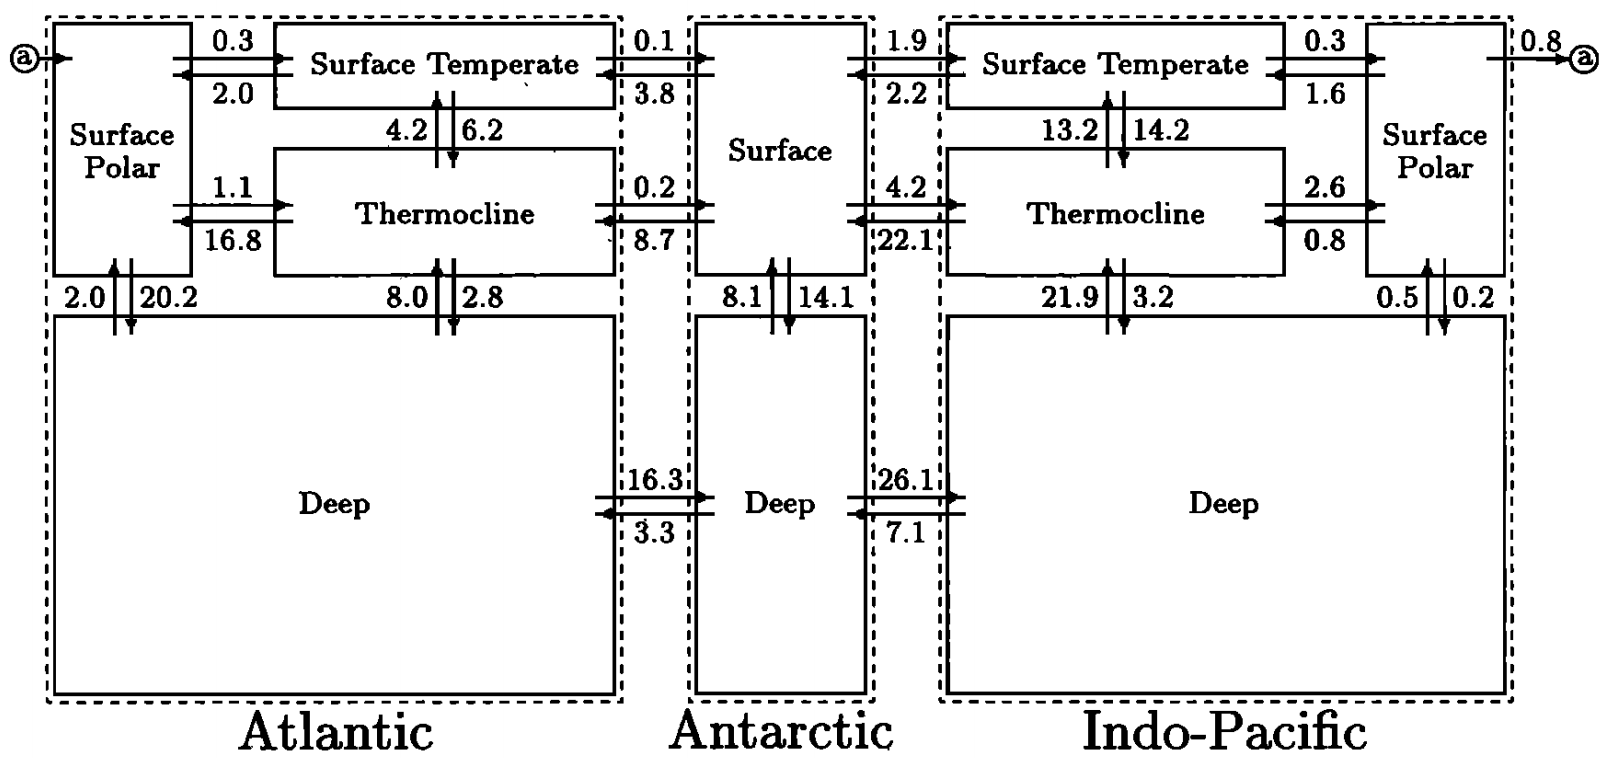
\includegraphics[width=\textwidth]{fig/intro/boxmodel_Munhoven.png}
		\caption{Geometry and water fluxes of a compartmental model for the World Ocean. The fluxes are expressed in sverdrups ($1$ Sv = $10^6$ $\rm{m^3/s}$). This is figure 3 of \cite{munhoven1996glacial}.}
	\end{subfigure}%
\caption{Schematic representations of different compartment models.}\label{fig:intro:boxmodels}
\end{figure}
\begin{figure}[!htp]
	\centering
	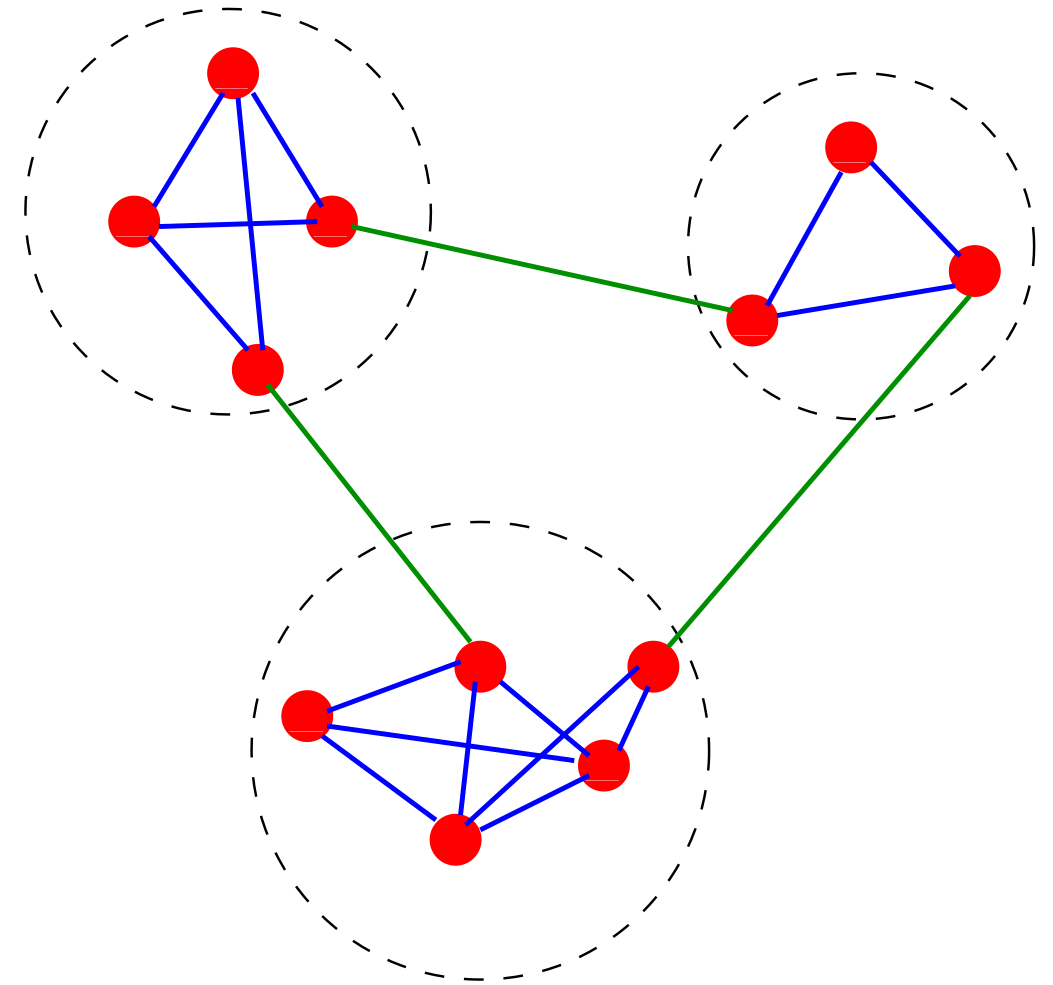
\includegraphics[width=.4\textwidth]{fig/intro/communities_example.png}
	\caption{Example of a three-communities partitioning on a simple network.} \label{fiug:intro:communities}
\end{figure}